%
% poissonproblem.tex
%
% (c) 2019 Prof Dr Andreas Mueller
%
\section{Poisson problem}
\rhead{Poisson problem}
\label{poisson-problem}
\begin{figure}
\centering
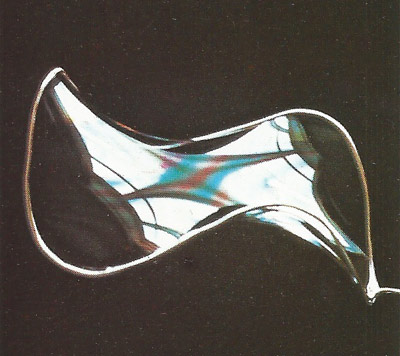
\includegraphics[width=0.4\hsize]{1-examples/images/minimum-area-surface.jpg}
\caption{The minimal surface realized by a soap film can be described as
the graph of a function $u(x,y)$ over a domain in the horizontal $x$-$y$-plane.
The boundary is given by the wire, which can be seen as boundary values
$f(x,y)$ for points $(x,y)$ on the boundary.
\label{examples:minimal-surface-image}}
\end{figure}
This section describes two examples of elliptic partial differential
equations, to be expanded on in chapter~\ref{chapter-elliptisch}.

\subsection{Minimal surfaces\label{beispiele:minimal surfaces}}
What shape will a soap film take when it is lifted to height
$f(x,y)$ at the boundary $(x,y)\in\gamma$ of 
a two dimensional domain $G\subset \mathbb R^2$
(see figure~\ref{examples:minimal-surface-image})?
If we describe the height of the soap film using a function
$u(x,y)$, we expect to find a partial differential equation for $u$
with boundary condition $f$.
\index{minimal surface}

In the derivation of the equation of motion for the vibrating string
we learned that the force accelerating the string depended on the
curvature of the string.
For the soap film, the restoring force is provided by the surface
tension which is equally strong in each direction of the film.
The soap film has two directions in which it can curve, roughly
given by the second partial derivatives $\partial^2 u/\partial x^2$ and
$\partial^2 u/\partial y^2$.
We therefore expect that force accelerating the film proportional
to the sum of these second derivatives with respect to $x$ and $y$.
Since the film is supposed not to move, we expect the differential
equation:
\[
\frac{\partial^2 u }{\partial x^2}+\frac{\partial^2 u }{\partial y^2}
=\Delta u =0.
\]

This simplified derivation is only valid for small deviations.
More generally, the so called mean curvature of the surface needs
to vanish for a minimal surface.
\index{mean curvature}

\subsection{Electric potential}
\index{electric potential}
In electrodynamics it is shown that a static electric field is a 
gradient field, i.~e.~there is a potential $\varphi$ such that the
electric field
\[
\vec E=\operatorname{grad}\varphi
\]
is its gradient.
It is also shown that the sources of the field are the electric charges.
Without charges, there are no sources to the field.
The mathematical expression of these facts is that 
the electric field satisfies the same partial differential equation
\[
\operatorname{div}\vec E=\operatorname{div}\operatorname{grad}\varphi
=\Delta \varphi=0
\]
as a minimal surface.
This problem seems to have mathematical significance independent of the
particular application.

